\chapter{Integration of Kramers--Kronig Architecture in Optical Inter-Satellite Link Model}

\section{Mathematical Derivation of KK-OISL Model}

\subsection{Optical Field Representation and Minimum-Phase Condition}

The Kramers--Kronig (KK) receiver needs a strong continuous-wave (CW) tone at the edge of the signal spectrum \cite{mecozzi2016}. In this model the tone (carrier) is generated at the \emph{transmitter} from the same laser and IQ modulator as the data, and travels with the data over the link. A baseband data signal $s(t)$ of symbol rate $B$, normalised to unit average power, is single-sideband (SSB) shifted to the right of the carrier:
\begin{equation}
E_{Tx}(t)=\Big[\sqrt{P_c}+\sqrt{P_s}\,s(t)\,e^{i2\pi f_{sh}t}\Big]e^{i\theta_L(t)},\qquad f_{sh}=B_o/2
\end{equation}
where $B_o=(1+\beta)B$ is the occupied bandwidth for a pulse roll-off $\beta$, $\theta_L(t)$ is the laser phase noise, $P_c$ is the carrier power and $P_s$ is the signal power. The SSB term occupies $[0,B_o]$, so the carrier lies at the lower edge of the signal spectrum.

The cross term $2\sqrt{P_cP_s}\,\mathrm{Re}\{s\,e^{i2\pi f_{sh}t}\}$ averages to zero, so the total transmit power is $P_T=P_c+P_s$. With the carrier-to-signal power ratio (CSPR) $\kappa=P_c/P_s$:
\begin{equation}
P_c=\frac{\kappa}{1+\kappa}P_T,\qquad P_s=\frac{1}{1+\kappa}P_T
\end{equation}
Only the fraction $1/(1+\kappa)$ of the transmit power carries data. This is the physical CSPR penalty.

At the receiver aperture both components are attenuated by the same total channel power gain $h=h_{PL}\,h_{PE}$:
\begin{equation}
E_{Rx}(t)=\sqrt{h}\Big[\sqrt{P_c}+\sqrt{P_s}\,s(t)\,e^{i2\pi f_{sh}t}\Big]e^{i\theta_L(t)+i\phi_D(t)}
\end{equation}
where $\phi_D(t)$ is the Doppler phase. Carrier and data come from the same laser and travel the same path in the same polarisation and spatial mode. The laser phase noise, the Doppler shift, any polarisation rotation and any wavefront tilt are therefore common to both and cancel in square-law detection (eq.~3.5). As a result:
\begin{itemize}
\item No local-oscillator frequency locking is needed. For a 550\,km LEO shell the carrier Doppler can reach $\pm9.9$\,GHz. Carrier and data are shifted almost equally; the data sideband, which lies $f_{sh}=5.25$\,GHz above the carrier, receives an extra shift of $f_{sh}v/c\approx263$\,kHz at $v=15$\,km/s, and the symbol clock is scaled by $v/c=50$\,ppm. Without correction these residuals destroy the link (SNR $\approx2$\,dB in the waveform simulation). A pilot-based frequency estimate, a clock correction derived from the same estimate ($\epsilon=\Delta f/f_{sh}$) and blind phase tracking remove them, with a penalty of at most 0.4\,dB down to the HD-FEC threshold.
\item No polarisation control is needed.
\item The CSPR at the receiver equals $\kappa$ for every pointing state.
\end{itemize}

For exact phase retrieval from intensity, $E_{Rx}(t)$ must be minimum phase. A sufficient condition is that the time trajectory of the field does not encircle the origin:
\begin{equation}
\sqrt{P_c}>\sqrt{P_s}\,|s(t)|_{\max}\quad\Longleftrightarrow\quad \kappa>\mathrm{PAPR}_s=\frac{\max|s(t)|^2}{\langle|s(t)|^2\rangle}
\end{equation}
\emph{Proof.} Put $u=\sqrt{P_s/P_c}\,s\,e^{i2\pi f_{sh}t}$, with $|u|<1$. Then $\ln(1+u)=\sum_n(-1)^{n+1}u^n/n$ contains only positive frequencies, so its imaginary part (the phase) is the Hilbert transform of its real part, $\ln|1+u|$ \cite{mecozzi2016}. \hfill$\square$

For root-raised-cosine (RRC) pulses with $\beta=0.05$, the PAPR, defined as the $10^{-4}$ point of the instantaneous-power CCDF ($2^{17}$ symbols), is about 7.5\,dB (BPSK), 7.4\,dB (OOK) and 6.4\,dB (QPSK). The largest peak of a single waveform is not used, because it depends on the random sequence. $\kappa=12$\,dB is used throughout; the noise model of Section~3.1.3 is verified for $\kappa\ge12$\,dB.

\subsection{Square-Law Detection and KK Phase Reconstruction}

A photodiode with responsivity $\eta$ performs square-law detection to produce the photocurrent $I(t)$:
\begin{equation}
I(t)=\underbrace{\eta hP_c}_{\text{Carrier DC Current}}+\underbrace{\eta hP_s|s(t)|^2}_{\text{Signal-Signal Beat Current}}+\underbrace{2\eta h\sqrt{P_cP_s}\,\mathrm{Re}\{s(t)e^{i2\pi f_{sh}t}\}}_{\text{Cross-Beat Signal Current}}+n(t)
\end{equation}
The common phases $\theta_L$ and $\phi_D$ have disappeared. The photocurrent is converted to power units by dividing by the responsivity only. No noise is subtracted, and no division by the unknown channel gain is needed:
\begin{equation}
I_n(t)=\frac{I(t)}{\eta}
\end{equation}
Under the minimum-phase condition, the optical phase $\phi_E(t)$ and the field envelope $\sqrt{I_n(t)}$ are uniquely related by the KK relation, through the Hilbert transform $\mathcal H\{\cdot\}$:
\begin{equation}
\phi_E(t)=\mathcal H\Big\{\tfrac12\ln I_n(t)\Big\}=\frac{1}{2\pi}\,\mathrm{P.V.}\!\int_{-\infty}^{\infty}\frac{\ln I_n(t')}{t-t'}\,dt'
\end{equation}
With the Fourier convention $\mathcal F\{x\}(f)=\int x(t)e^{-i2\pi ft}dt$ (as used by MATLAB \texttt{fft}), the phase reconstruction in the frequency domain is:
\begin{equation}
\tilde\phi_E(f)=-i\cdot\mathrm{sgn}(f)\cdot\mathcal F\Big\{\tfrac12\ln I_n(t)\Big\}
\end{equation}
The complex envelope is reconstructed as:
\begin{equation}
\hat E(t)=\sqrt{I_n(t)}\,e^{i\phi_E(t)}=\sqrt h\Big[\sqrt{P_c}+\sqrt{P_s}\,s(t)\,e^{i2\pi f_{sh}t}\Big]
\end{equation}
The received carrier is the time average $\hat a=\langle\hat E(t)\rangle=\sqrt{hP_c}$. It is removed, and \emph{then} the result is frequency down-shifted:
\begin{equation}
\hat E_s(t)=\big[\hat E(t)-\hat a\big]e^{-i2\pi f_{sh}t}=\sqrt{hP_s}\;s(t)
\end{equation}
The signal-signal beat current is removed exactly by this reconstruction; it does not have to be negligible. For a transmitted signal $s(t)=\sum_k a_k\,p(t-kT)$, matched filtering with $p(t)$ and sampling at symbol period $T$ gives:
\begin{equation}
y_k=\big(\hat E_s\ast p\big)(kT)\approx\sqrt{hP_s}\,a_k
\end{equation}
\begin{equation}
\hat a_k=\arg\min_{c}\,|y_k-\sqrt{hP_s}\,c|,\qquad \text{e.g. BPSK: }\hat a_k=\mathrm{sgn}[\mathrm{Re}(y_k)]
\end{equation}
No carrier-phase recovery is needed, because the transmitted carrier is the phase reference.

\subsection{Physical Receiver Noise Budget and Electrical SNR Model}

The receiver is a PIN photodiode with thermal noise. An optional optical pre-amplifier (EDFA with fixed gain $G$, noise figure $F$ and an optical band-pass filter of width $B_f$) can be placed before it; without the pre-amplifier, $G=1$. The carrier and signal powers at the photodiode are $P_{c,d}=G\frac{\kappa}{1+\kappa}h_{PL}\,y\,P_T$ and $P_{s,d}=G\frac{1}{1+\kappa}h_{PL}\,y\,P_T$, where $y=h_{PE}$. The cross-beat electrical signal power is:
\begin{equation}
S(y)=2\eta^2P_{c,d}P_{s,d}=2\eta^2G^2h_{PL}^2P_T^2\,y^2\,\frac{\kappa}{(1+\kappa)^2}
\end{equation}

\emph{KK noise mapping.} Linearising eqs.~(3.7)--(3.9) for a small photocurrent noise $w$ (in W) gives the field error $\delta=\tfrac12\hat E\,\mathcal A\{w/|\hat E|^2\}$, where $\mathcal A\{x\}=x+i\mathcal H\{x\}$. For large $\kappa$ this reduces to $\delta\approx\mathcal A\{w\}/(2\sqrt{P_{c,d}})$. A photocurrent noise of one-sided power spectral density (PSD) $N_i$ [A$^2$/Hz] therefore gives a symbol SNR $g_i=S/(\zeta N_iB)$. The factor
\[
\zeta=1+2/\kappa
\]
is the second-order KK noise enhancement; it was checked by waveform simulation to within 0.15\,dB for $\kappa\ge12$\,dB (0.8\,dB at $\kappa=9$\,dB and 4.7\,dB at 6\,dB).

\emph{ASE noise.} The amplified spontaneous emission (ASE) PSD per polarisation is $S_{ASE}=h\nu(FG-1)/2$. ASE lying on both sides of the carrier beats with it into the same band, the left half appearing as an image. The ASE limit is therefore $g_{ASE}=P_{s,d}/[(1+\zeta)S_{ASE}B]$. The optical filter width $B_f=30$\,GHz accommodates the occupied bandwidth plus the Doppler range: $B_o+2\times9.9\,\mathrm{GHz}\approx30.3$\,GHz.

The receiver noise power spectral densities are:

\begin{itemize}
\item \textbf{Shot Noise:} $N_{sh}=2q\eta\,(P_{c,d}+P_{s,d}+2S_{ASE}B_f)$
\item \textbf{Front-End Thermal Noise:} $N_{th}=i_{th}^2$
\item \textbf{Transmit-Laser Relative Intensity Noise (RIN):} $N_{rin}=\mathrm{RIN}\cdot\eta^2(P_{c,d}+P_{s,d})^2$
\item \textbf{ASE$\times$ASE Beat (pre-amplifier, both polarisations):} $N_{aa}=4\eta^2S_{ASE}^2(B_f-B/2)$
\end{itemize}

\emph{KK reconstruction penalty (heuristic, not used).} The linear noise-mapping analysis above assumes the minimum-phase condition $\kappa>\mathrm{PAPR}_s$ holds at every instant. When $\kappa$ approaches or falls below $\mathrm{PAPR}_s$, the intensity $I_n(t)$ in eq.~(3.7) reaches near-zero values; the logarithm amplifies these events into large phase errors that are not captured by the first-order expansion. A simple closed-form attempt is to add an inverse-SNR term set by the probability that a Gaussian approximation of the signal envelope violates the minimum-phase condition:
\begin{equation}\label{eq:recon}
\frac{1}{g_{recon}}=\mathrm{PAPR}_s\cdot P_{viol}(\kappa),\qquad P_{viol}=\begin{cases}e^{-\kappa}&\text{QPSK (complex Gaussian)}\\[4pt]\mathrm{erfc}\!\big(\!\sqrt{\kappa/2}\big)&\text{BPSK, OOK (real Gaussian)}\end{cases}
\end{equation}
For QPSK, $s(t)$ is treated as circularly symmetric complex Gaussian, so $P_{viol}=\Pr(|s|^2>\kappa)=e^{-\kappa}$; for BPSK and OOK, $s(t)$ is treated as real Gaussian, $P_{viol}=\Pr(|s|>\sqrt\kappa)=\mathrm{erfc}(\sqrt{\kappa/2})$. The waveform simulation of Section~3.2 shows that this term is 35--50\,dB too pessimistic: with all noise switched off, KK reconstruction of QPSK reaches 44.8, 78.2 and 100.9\,dB SNR at $\kappa=6$, 9 and 12\,dB, where the formula predicts 10.5, 27.7 and 62.0\,dB. The Gaussian approximation counts how often the envelope exceeds the carrier but not how strongly the occasional, very short violations disturb the reconstructed field. The term is therefore \emph{not} included in the results; the code keeps it as an option (\texttt{P.recon}) for comparison, and the optimum CSPR is determined by waveform simulation.

The SNR contribution of each noise is:
\begin{equation}
g_j(y)=\frac{S(y)}{\zeta\,N_j\,B}\quad(j=sh,th,rin,aa),\qquad g_{ASE}(y)=\frac{P_{s,d}}{(1+\zeta)S_{ASE}B}
\end{equation}
The independent noise powers add, so the total average electrical SNR as a function of the pointing fraction $y$ is:
\begin{equation}
g(y)=\bigg(\sum_j\frac{1}{g_j(y)}+\frac{1}{g_{recon}}\bigg)^{\!-1}
\end{equation}
where the sum runs over $j\in\{sh,th,rin,ASE,aa\}$ (the last two only with the pre-amplifier). The heuristic term $1/g_{recon}$ of eq.~(\ref{eq:recon}) is omitted (see above).

Without the pre-amplifier, the thermal term scales as $y^{-2}$, because the carrier arrives as weak as the data and the receiver has no local-oscillator gain. With the pre-amplifier, the ASE term ($\propto y^{-1}$) dominates near the beam axis, but below $y\approx0.02A_0$ the thermal term dominates again (Fig.~3.4). Deep fades, where outages occur, are therefore thermal-noise limited even with the EDFA.

The CSPR enters the photocurrent-noise terms as $\kappa/(1+\kappa)^2$ and the ASE term as $1/(1+\kappa)$. Raising $\kappa$ moves power from the data to the carrier and lowers the SNR; lowering it towards $\mathrm{PAPR}_s$ makes KK reconstruction degrade. The optimum lies in between. Because the analytic model is verified only for $\kappa\ge12$\,dB and the heuristic reconstruction term is unreliable, the optimum is found from the waveform simulation (Section~3.2).

\subsection{Pointing Error Statistics and Fading Distribution}

For a Gaussian optical beam with waist $w_0$ at frequency $f=c/\lambda$, the relevant quantities are:
\begin{itemize}
\item beam radius at distance $z$: $w_z=z\tan\!\big(\tfrac{c}{\pi fw_0}\big)$;
\item peak collected power fraction: $A_0=\frac{2w_d^2}{w_z^2}$;
\item distance-dependent pointing jitter variance: $\sigma_s^2(z)=\sigma_{s0}^2\exp\!\big(\tfrac{2k_0z}{d_0}\big)$.
\end{itemize}
The pointing shape parameter $\alpha$ is:
\begin{equation}
\alpha=\frac{w_z^2}{4\sigma_s^2}
\end{equation}
The radial pointing deviation is Rayleigh distributed. The pointing loss fraction $y\in(0,A_0]$ then follows a power-law probability density function (PDF) and cumulative distribution function (CDF):
\begin{equation}
f_Y(y)=\frac{\alpha}{A_0^\alpha}y^{\alpha-1},\qquad F_Y(y)=\Big(\frac{y}{A_0}\Big)^{\alpha},\qquad 0<y\le A_0
\end{equation}

\subsection{Achievable Data Rate Integration}

The hard-decision information rate per symbol $m_i(g)$ [bits/symbol] as a function of SNR $g=E_s/N_0$ is formulated using the binary entropy:
\begin{equation}
H_2(p)=-p\log_2(p)-(1-p)\log_2(1-p)
\end{equation}
\begin{itemize}
\item \textbf{BPSK (1 bit/symbol):} $m_{BPSK}(g)=1\cdot\big[1-H_2\big(Q(\sqrt{2g})\big)\big]$
\item \textbf{OOK (1 bit/symbol):} $m_{OOK}(g)=1\cdot\big[1-H_2\big(Q(\sqrt{g})\big)\big]$. OOK is BPSK at $g/2$, because half of its energy is a data-free tone.
\item \textbf{QPSK (2 bits/symbol):} $m_{QPSK}(g)=2\cdot\big[1-H_2\big(Q(\sqrt{g})\big)\big]$
\end{itemize}
where $Q(x)=\frac12\mathrm{erfc}\big(x/\sqrt2\big)$.

The soft-decision rates are evaluated by Gauss--Hermite quadrature. For BPSK,
\[
m^{s}_{BPSK}(g)=1-\mathbb E_z\log_2\!\big(1+e^{-4g(1+z/\sqrt{2g})}\big),\qquad z\sim\mathcal N(0,1),
\]
and $m^s_{OOK}(g)=m^s_{BPSK}(g/2)$, $m^s_{QPSK}(g)=2m^s_{BPSK}(g/2)$. These are upper bounds on the hard-decision rates.

Integrating over the pointing fading distribution gives the ergodic achievable rate $R_{KK}$ [bits/s]:
\begin{equation}
R_{KK}=\int_{0}^{A_0}B\cdot m_i\big(g(y)\big)\,f_Y(y)\,dy
\end{equation}
No detector threshold is imposed; the rate falls off through $g(y)$ itself. If a tracking threshold power $p_{th}$ is to be modelled, the lower limit becomes $y_{th}=p_{th}/(h_{PL}P_T)$, which is dimensionless. Applying the logarithmic change of variable $t=\ln y$ ($y=e^t$, $dy=e^tdt$) yields the exact computational form:
\begin{equation}
R_{KK}=B\int_{-\infty}^{\ln A_0}m_i\big(g(e^t)\big)\cdot\alpha\exp\big(\alpha(t-\ln A_0)\big)\,dt
\end{equation}

Pointing jitter is slow compared with a codeword, so the rate guaranteed for all but a fraction $\epsilon$ of the time is also reported. It follows in closed form from $F_Y$:
\begin{equation}
R_\epsilon=B\cdot m_i\big(g(A_0\,\epsilon^{1/\alpha})\big)
\end{equation}
The receiver sensitivity is the received power at which the BER reaches the 7\,\% hard-decision forward error correction (FEC) threshold of $3.8\times10^{-3}$. This requires $g^\star=5.5$\,dB for BPSK and $8.5$\,dB for QPSK and OOK.

\section{Simulation and Results}

\begin{table}[h]
\centering
\caption{DEFAULT PARAMETERS SETUP II}
\begin{tabular}{|l|l|l|}
\hline
\textbf{Parameter} & \textbf{Value} & \textbf{Description}\\\hline
$w_0$ & 0.1\,m & beam waist at TX\\\hline
$w_d$ & 0.07\,m & detector radius (30\,\% smaller than $w_0$)\\\hline
$f_{default}$ & 195.94\,THz (1530\,nm) & default frequency (ITU-T C-band short edge)\\\hline
$h_{PL}$ & 0.9 & deterministic path loss\\\hline
$\eta$ & 0.5\,A/W & detector responsivity\\\hline
$P_{T,default}$ & 0.3\,W & total transmit power (carrier + signal)\\\hline
$\kappa$ & 12\,dB & CSPR at transmitter\\\hline
$B$ & 10\,GHz & symbol rate / bandwidth (RRC, $\beta=0.05$)\\\hline
$i_{th}$ & 20\,pA/$\sqrt{\text{Hz}}$ & thermal noise current density\\\hline
RIN & $-150$\,dB/Hz & transmit-laser RIN\\\hline
$G$, $F$, $B_f$ & 15\,dB, 5\,dB, 30\,GHz & pre-amplifier gain, noise figure, optical filter\\\hline
$z$ & 1000\,km & link distance\\\hline
$\sigma_{S0};k_0;d_0$ & 2; 0.1; 100e3 & $\sigma_s$ model, paper given values\\\hline
\end{tabular}
\end{table}

\begin{table}[h]
\centering
\caption{Noise Budget at $y=A_0$ ($A_0=4.132\times10^{-4}$, $w_z=4.870$\,m, $\alpha=0.201$)}
\begin{tabular}{|l|l|}
\hline
Received power (carrier / signal) & $-9.52$\,dBm ($-9.79$ / $-21.79$\,dBm)\\\hline
KK noise factor $\zeta$ & 1.126\\\hline
SNR (shot only) & 47.4\,dB\\\hline
SNR (thermal only) & 48.9\,dB\\\hline
SNR (RIN only) & 40.0\,dB\\\hline
SNR (signal/carrier--ASE only) & 31.9\,dB\\\hline
SNR (ASE$\times$ASE only) & 74.8\,dB\\\hline
KK reconstruction (QPSK, waveform, noiseless) & 100.9\,dB (negligible)\\\hline
SNR (total, on-axis, pre-amp) & 31.1\,dB\\\hline
SNR (total, photodiode only, no pre-amp) & 18.6\,dB\\\hline
Sensitivity BPSK / QPSK (pre-amp) & $-30.4$ / $-28.6$\,dBm\\\hline
\end{tabular}
\end{table}

\paragraph{Worked check of Table 3.2.} At $y=A_0$ the received power is $h_{PL}P_TA_0=0.9\times0.3\times4.132\times10^{-4}=1.116\times10^{-4}$\,W, i.e.\ $-9.52$\,dBm. Of this, $\kappa/(1+\kappa)=0.941$ is carrier. With the photodiode alone:
\begin{itemize}
\item cross-beat signal power: $S=2(0.5)^2(1.050\times10^{-4})(6.624\times10^{-6})=3.478\times10^{-10}$\,A$^2$;
\item thermal noise power: $\zeta i_{th}^2B=1.126\times4\times10^{-22}\times10^{10}=4.50\times10^{-12}$\,A$^2$;
\item ratio: $77.2$, i.e.\ $18.9$\,dB.
\end{itemize}
With the 15\,dB pre-amplifier the thermal SNR rises by $2\times15$\,dB to $48.9$\,dB, and the receiver becomes ASE limited ($31.9$\,dB).

\begin{figure}[h]
\centering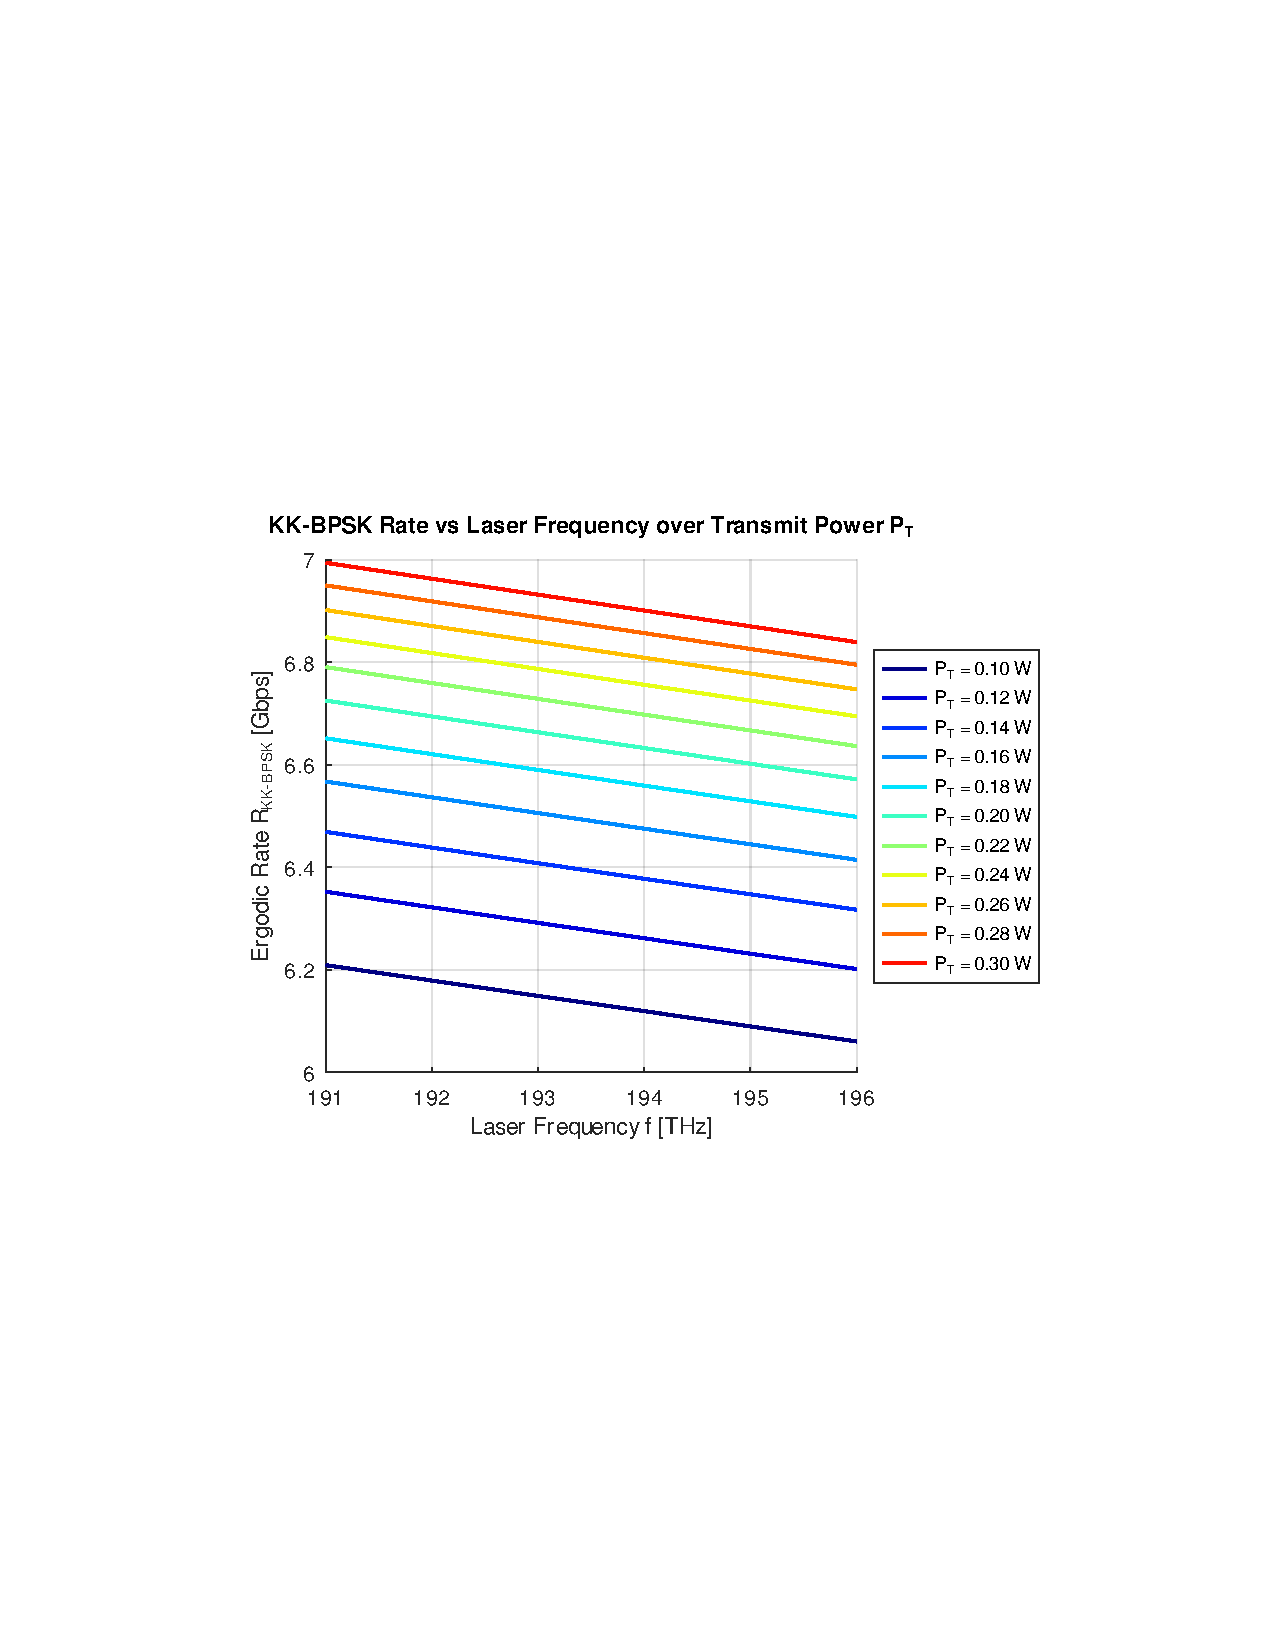
\includegraphics[width=0.85\textwidth]{figs/fig31.pdf}
\caption{BPSK Data Rate vs frequency}
\end{figure}

\begin{figure}[h]
\centering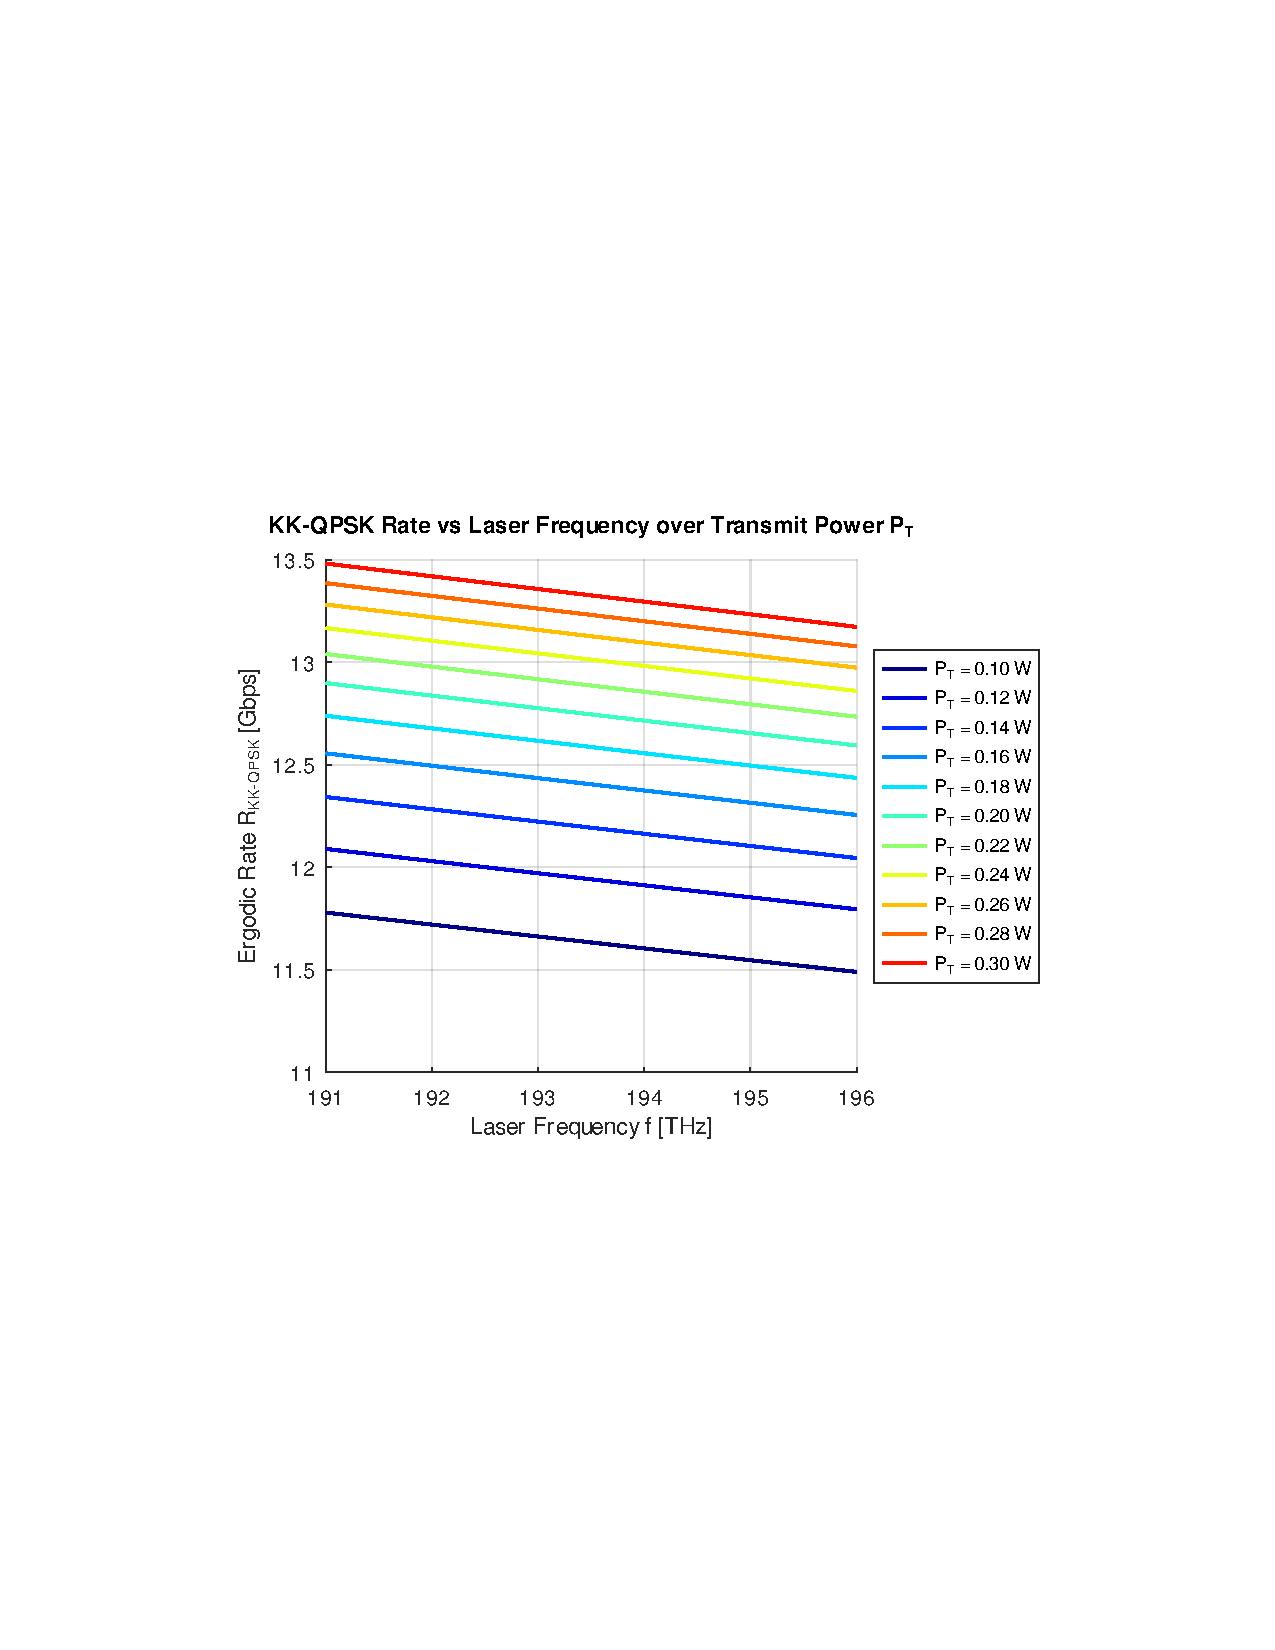
\includegraphics[width=0.85\textwidth]{figs/fig32.pdf}
\caption{QPSK Data Rate vs frequency}
\end{figure}

\begin{figure}[h]
\centering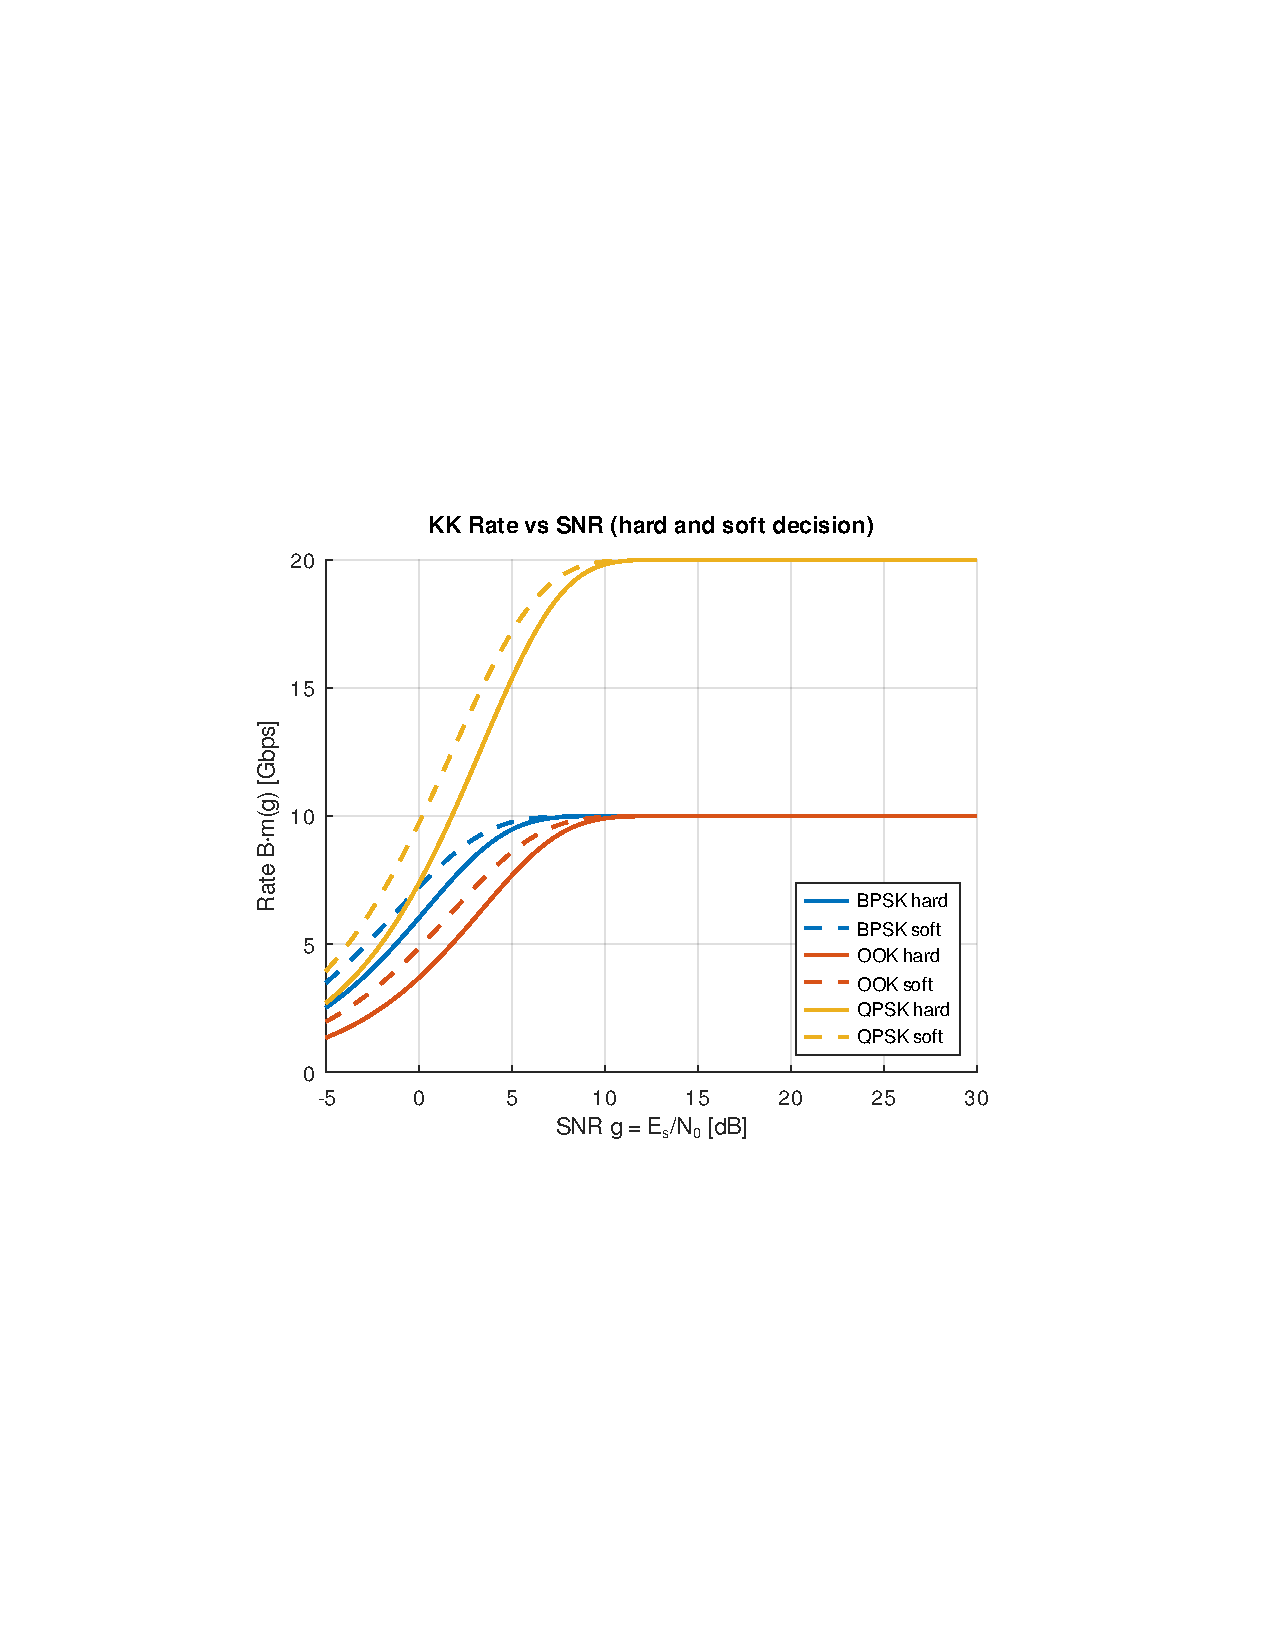
\includegraphics[width=0.85\textwidth]{figs/fig33.pdf}
\caption{Data Rate vs SNR (solid: hard decision, dashed: soft decision)}
\end{figure}

\begin{figure}[h]
\centering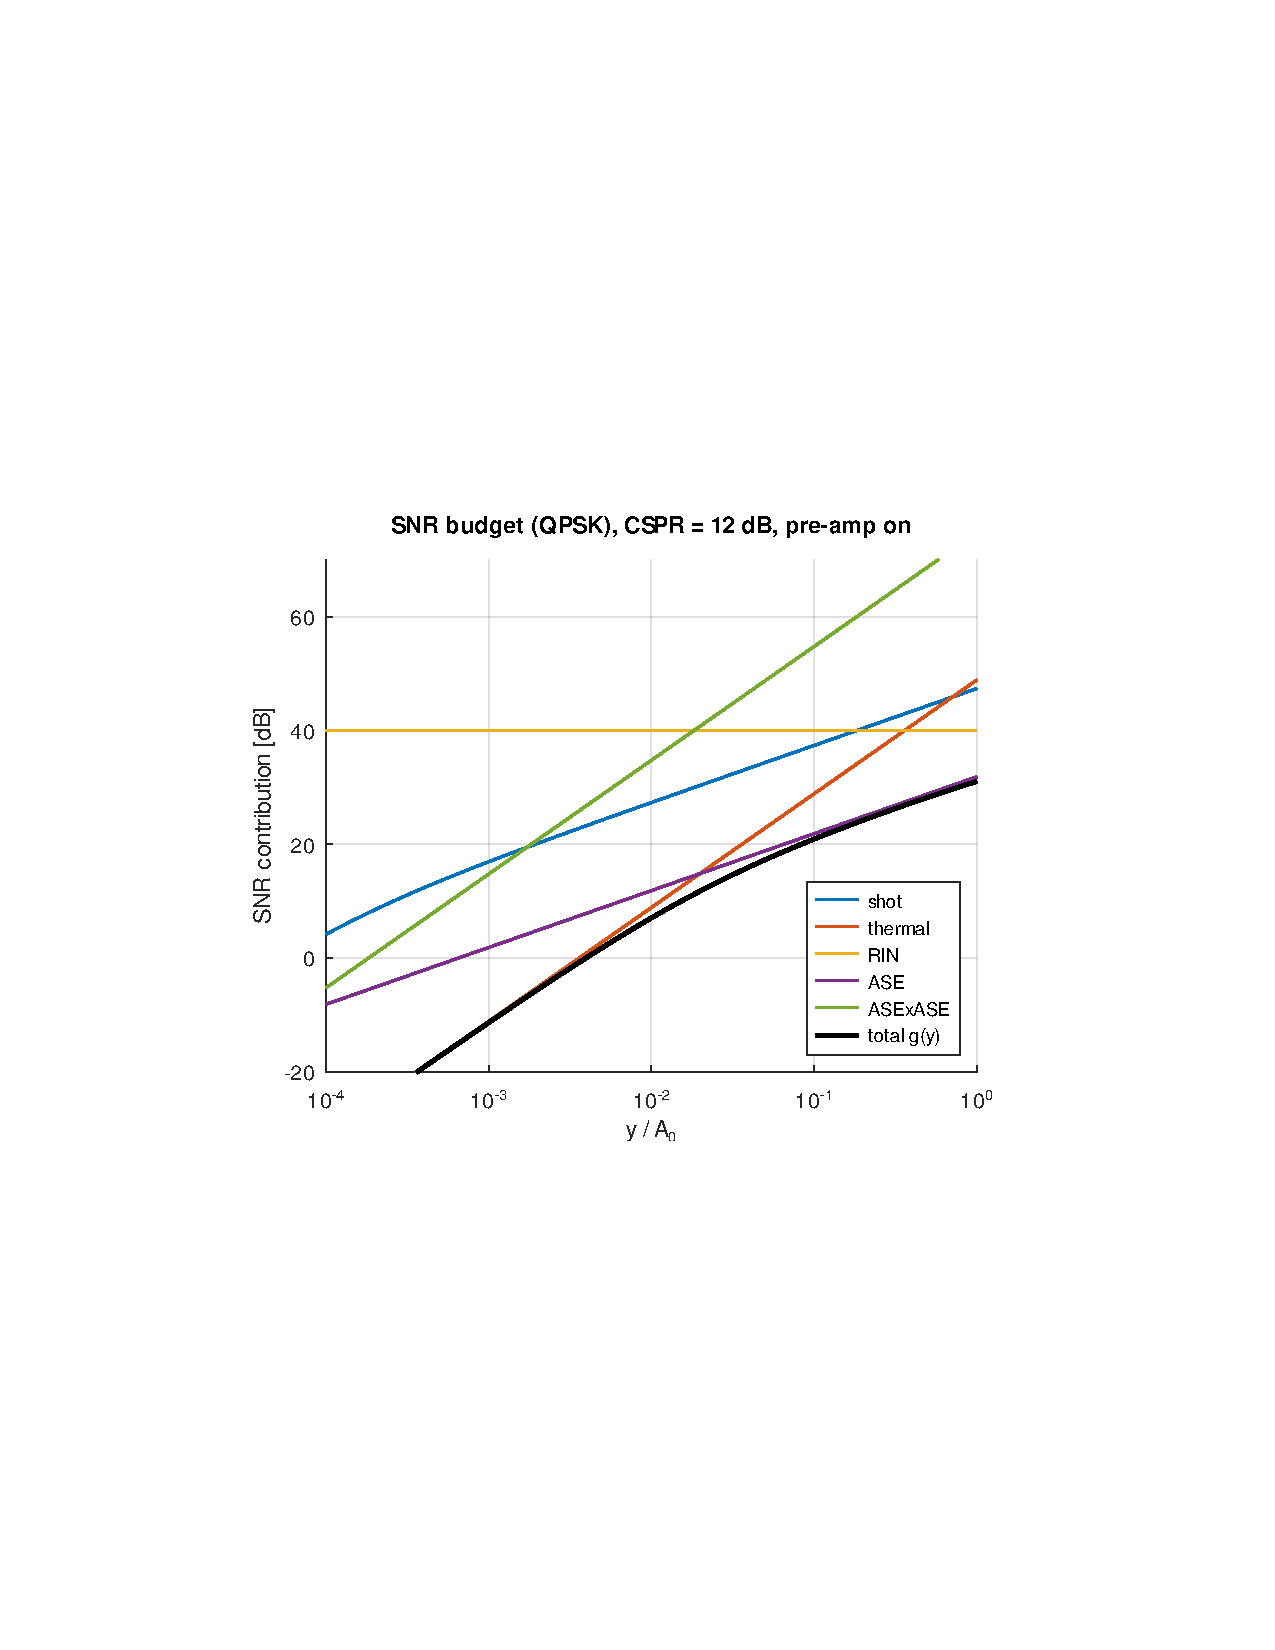
\includegraphics[width=\textwidth]{figs/fig34.pdf}
\caption{SNR contributions vs pointing fraction $y$ (QPSK, $\kappa=12$\,dB)}
\end{figure}

\begin{figure}[h]
\centering
\begin{subfigure}{0.48\textwidth}\centering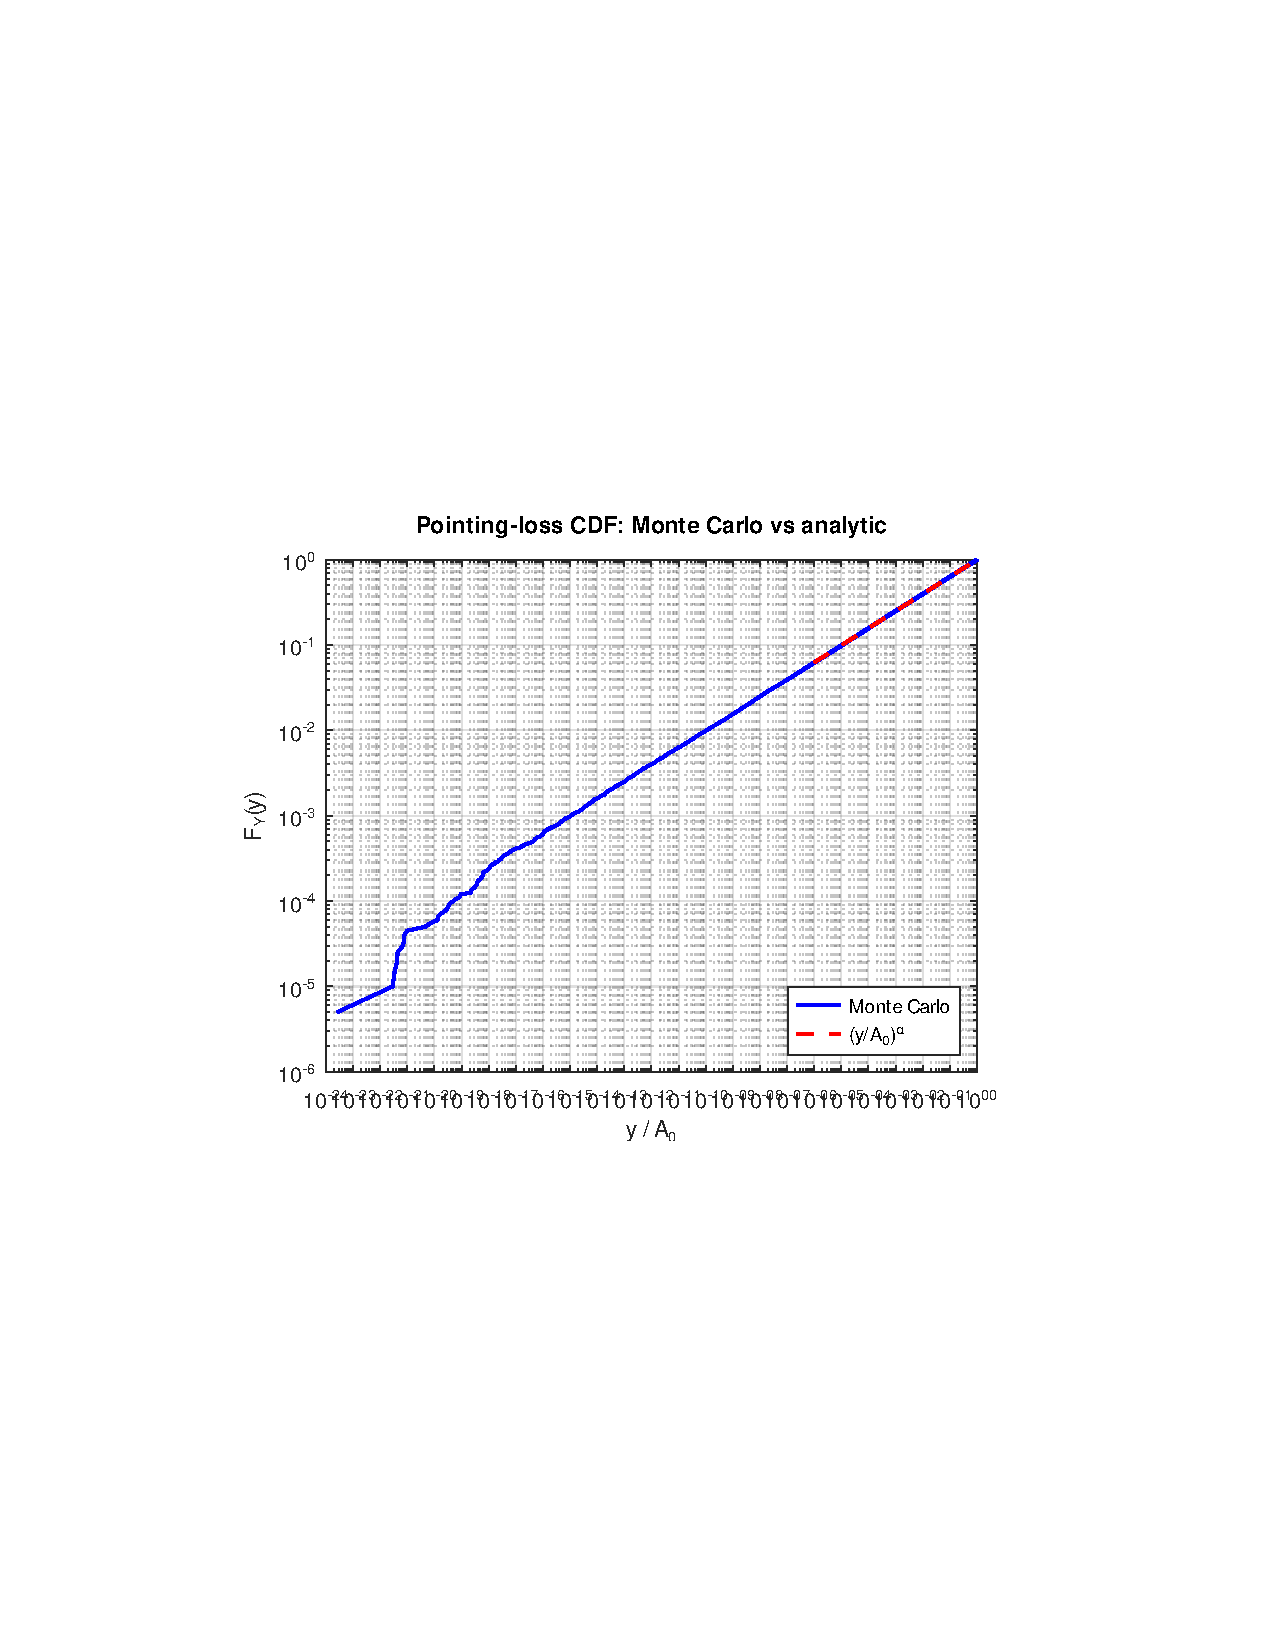
\includegraphics[width=\textwidth]{figs/fig35a.pdf}\caption{}\end{subfigure}\hfill
\begin{subfigure}{0.48\textwidth}\centering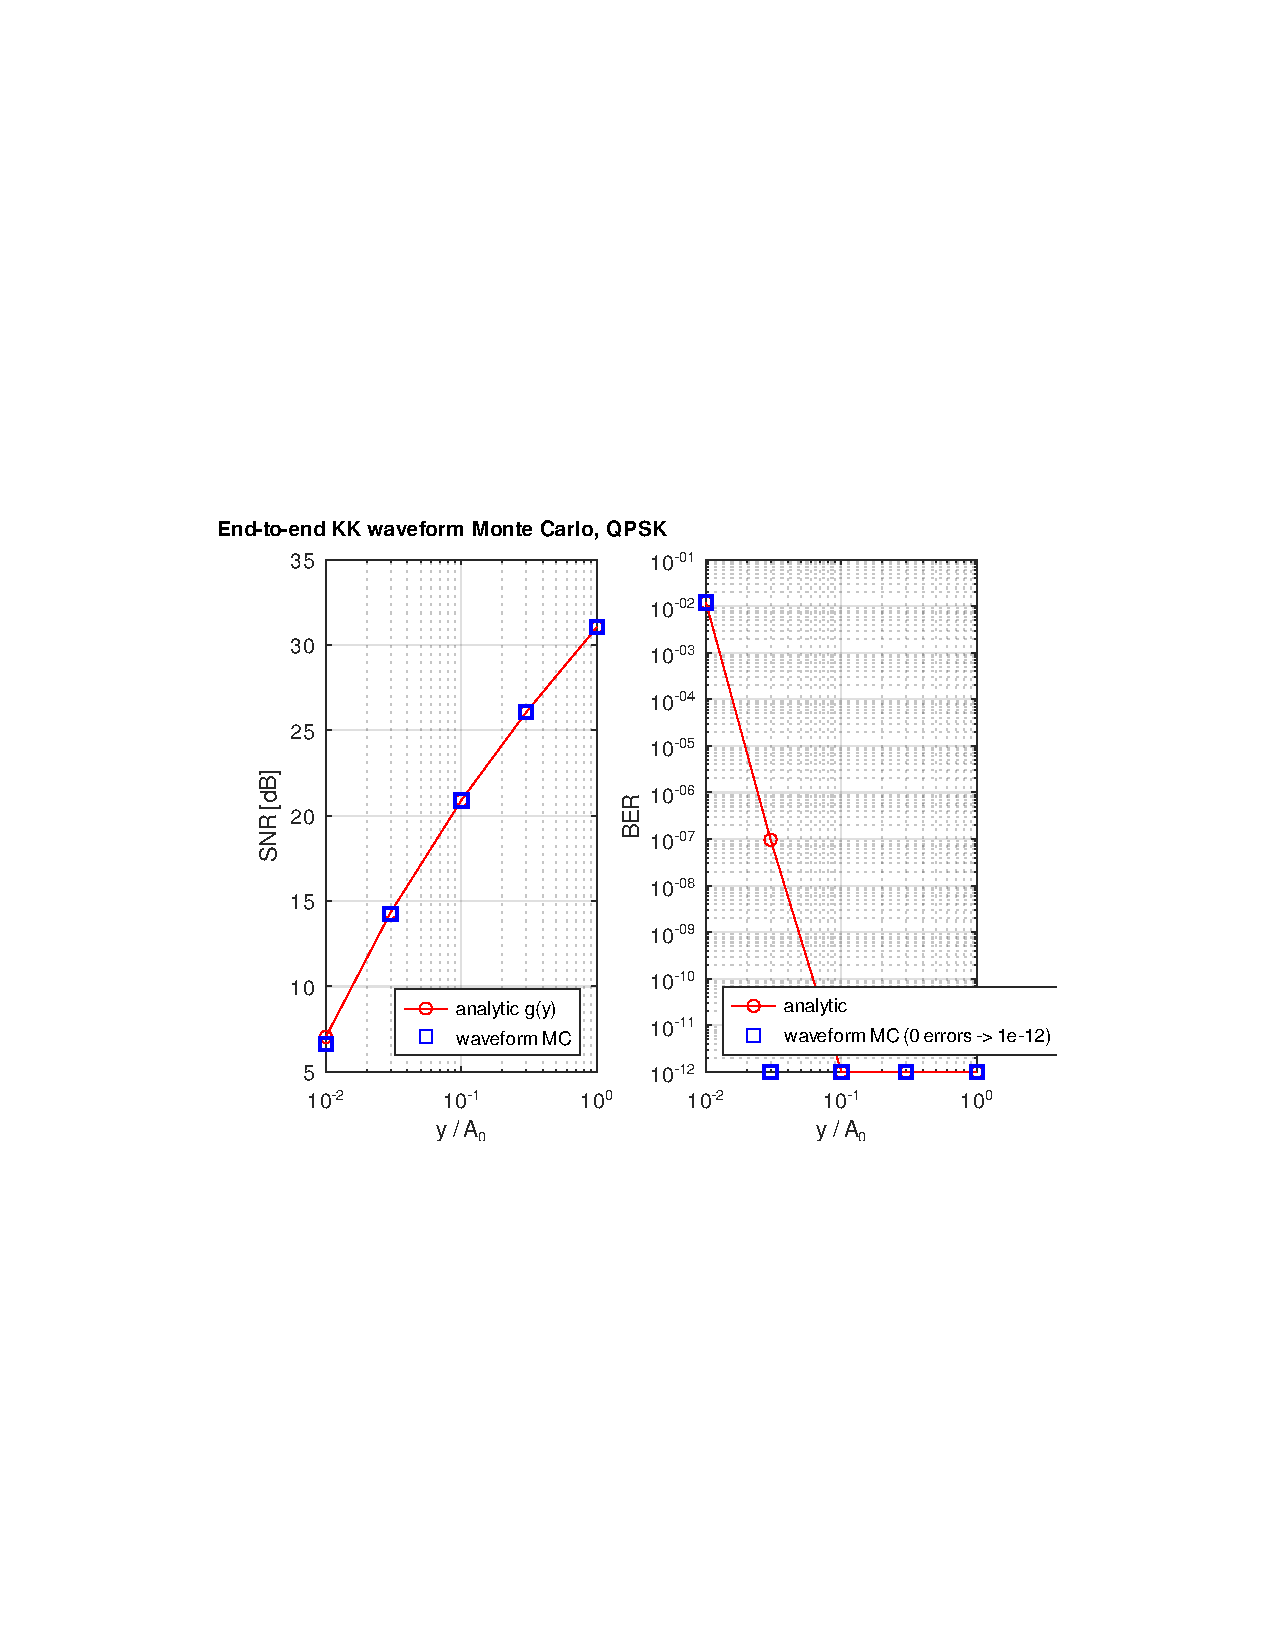
\includegraphics[width=\textwidth]{figs/fig35b.pdf}\caption{}\end{subfigure}
\caption{Monte Carlo validation: (a) pointing-loss CDF from $2\times10^5$ Rayleigh samples; (b) end-to-end KK waveform simulation ($2^{13}$ symbols per point, 512 pilots) vs analytic $g(y)$, QPSK}
\end{figure}

\paragraph{Ergodic rates.} At 195.94\,THz (1530\,nm) and $P_T=0.3$\,W, with the pre-amplifier, the ergodic rates are:
\begin{itemize}
\item BPSK: $6.84$\,Gbps (hard decision) / $6.96$\,Gbps (soft decision);
\item OOK: $6.59$ / $6.72$\,Gbps;
\item QPSK: $13.18$ / $13.44$\,Gbps.
\end{itemize}
Without the pre-amplifier they fall to $3.80$ (BPSK) and $6.70$\,Gbps (QPSK, hard decision).

\paragraph{Monte Carlo validation.} Averaging $B\,m(g(y))$ over the $2\times10^5$ channel samples gives 13.19\,Gbps for QPSK, matching the integral (13.18\,Gbps). The end-to-end waveform simulation (RRC pulses, carrier plus SSB signal, ASE in both polarisations, square-law photodiode with shot, thermal and RIN noise, KK DSP, matched filter and a 512-symbol pilot estimate) agrees with the analytic $g(y)$ within 0.1\,dB from $y=A_0$ to $y=0.03A_0$; at $y=0.01A_0$ (SNR $\approx7$\,dB) the waveform is 0.4\,dB lower, because the KK logarithm amplifies noise when the photocurrent approaches zero. With $2^{13}$ symbols, bit errors are observed only at $y=0.01A_0$ (BER $1.20\times10^{-2}$ measured vs $1.22\times10^{-2}$ analytic); at the other points the validation rests on the measured SNR.

For the photodiode-only receiver at low SNR, the photocurrent noise approaches the carrier level. The KK logarithm then amplifies it, and the analytic rate becomes an upper bound. This can be checked with the waveform Monte Carlo by setting \texttt{pre\_on=false}.

\paragraph{CSPR optimisation.} Fig.~\ref{fig:csprwave} shows the waveform SNR as a function of $\kappa$ for three pointing states, together with the analytic model. The optimum is $\kappa^\star\approx7$\,dB at $y=A_0$ and $0.1A_0$ (34.2 and 23.3\,dB, against 31.1 and 20.9\,dB at 12\,dB) and $\kappa^\star\approx9$\,dB at $y=0.03A_0$ (16.2 vs 14.3\,dB). Operating at the optimum gains 2--3\,dB; the optimum moves to higher $\kappa$ in deep fades. Below the optimum the analytic model, which does not capture KK breakdown, overestimates the SNR. The measured optimum of Wen \emph{et al.}~\cite{wen2023}, 7--8\,dB, agrees. This report keeps $\kappa=12$\,dB, where the noise model is verified.

\begin{figure}[h]
\centering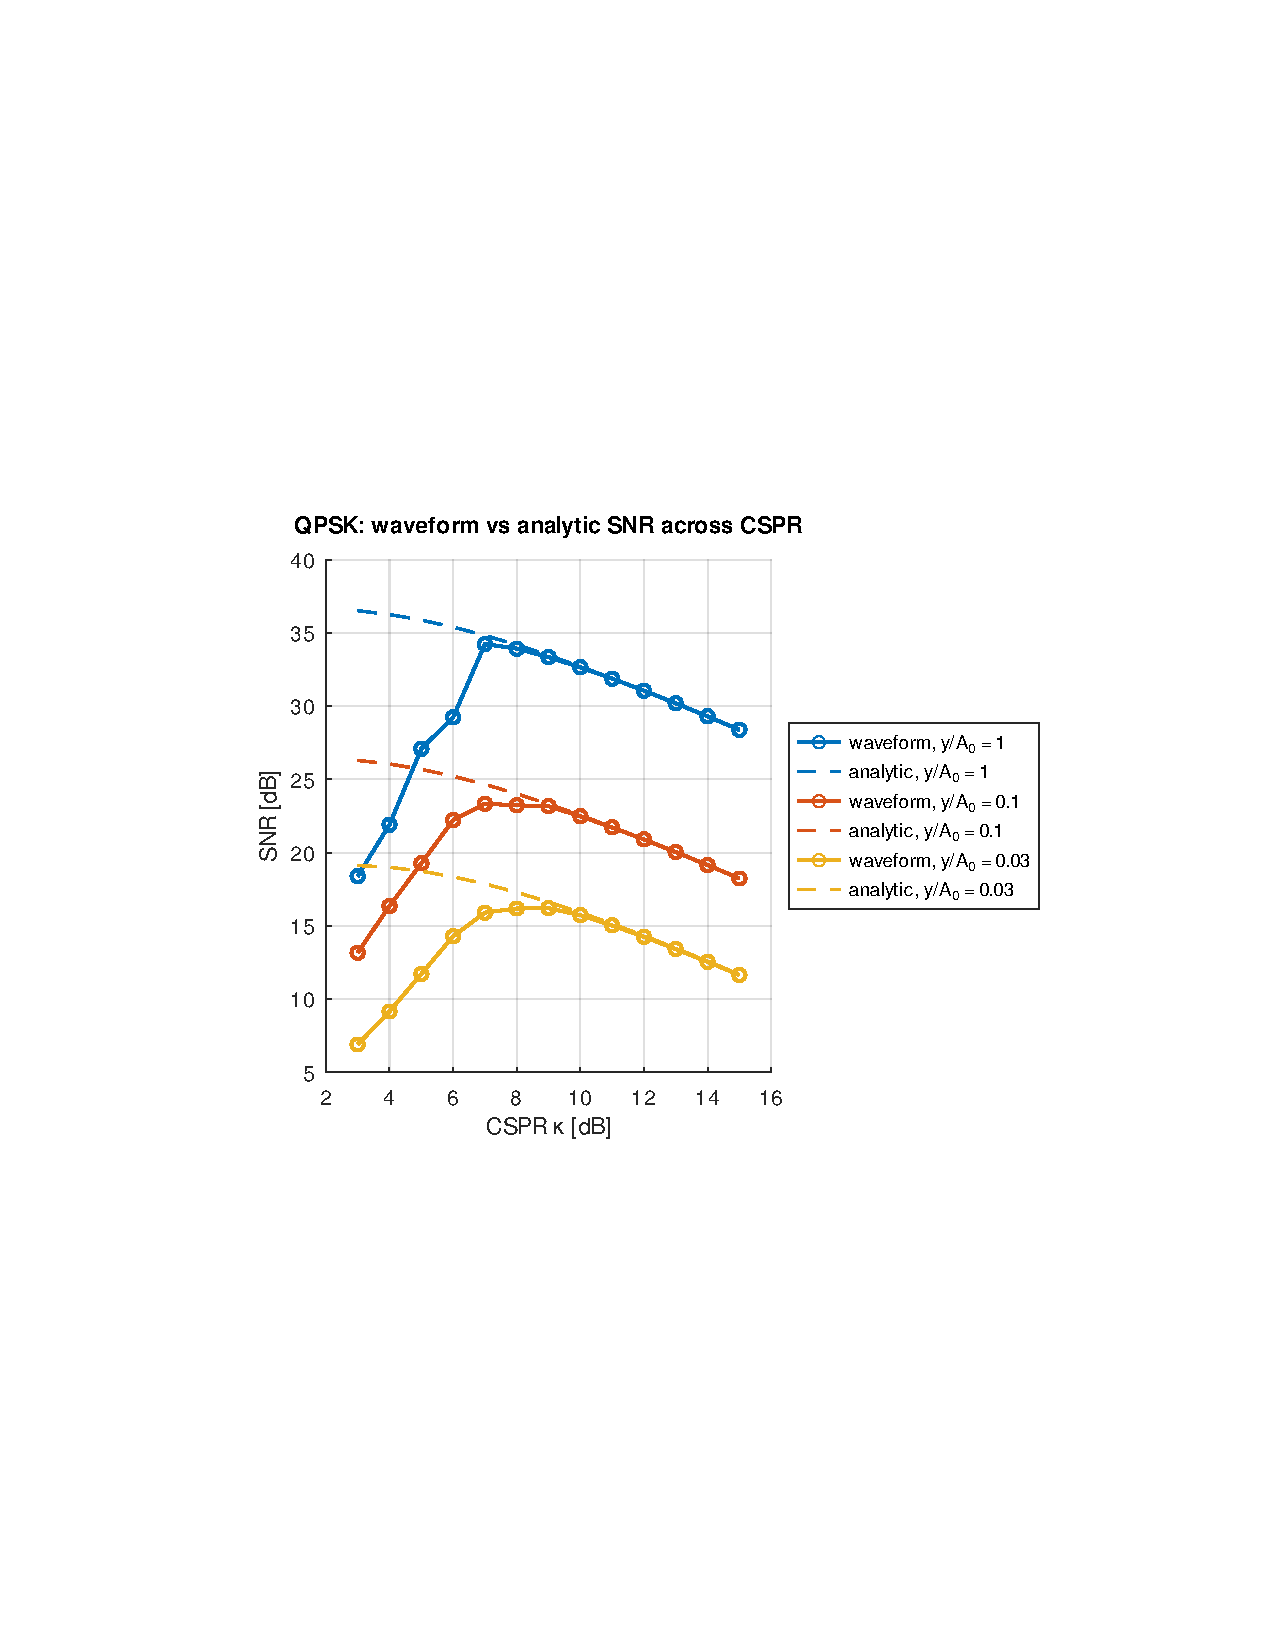
\includegraphics[width=0.85\textwidth]{figs/fig_cspr_wave.pdf}
\caption{QPSK SNR vs CSPR: waveform simulation (solid) and analytic model (dashed) at $y/A_0=1$, 0.1 and 0.03.}\label{fig:csprwave}
\end{figure}

\paragraph{Outage.} The $\epsilon$-outage rate is effectively zero for $\epsilon=0.1$ ($R_{0.1}\approx7.6\times10^{-5}$\,Gbps). Under the jitter model, $\sigma_s=5.44$\,m exceeds the beam radius $w_z=4.87$\,m at 1000\,km, so $\alpha=0.20$. With the smaller detector radius $w_d=0.07$\,m, $A_0=4.13\times10^{-4}$ and the link spends 41\,\% of the time below the QPSK sensitivity even with the pre-amplifier. Pointing jitter, not the KK receiver, limits reliability.

\subsection{Constellation Analysis: Carrier Placement Configurations}

To demonstrate \emph{why} the carrier must co-propagate with the data, four carrier/LO configurations are simulated at $y=A_0$ for QPSK with $2^{13}$ symbols. All four use the same waveform chain; the gain and phase are estimated from 512 pilot symbols, and SNR, EVM, BER and phase error are measured on the remaining 7680 symbols.

\begin{itemize}
\item \textbf{A2 (TX Carrier):} The standard configuration used throughout this chapter. The carrier co-propagates with the signal through the channel, undergoes the same fading and phase rotation, and arrives at the photodiode in phase with the data.

\item \textbf{B1 (RX Optical LO):} The transmitter sends only the SSB data signal at full power $P_T$. A local CW laser of 1.77\,mW (CSPR 12\,dB at $y=A_0$) is combined with the incoming signal \emph{before} the photodiode; no EDFA is used, since the LO provides the gain. The LO is ideal: no frequency offset, no linewidth and matched polarisation.

\item \textbf{A1/B3 (No Carrier):} The signal is transmitted and received alone, with no carrier from either end. The KK algorithm attempts phase retrieval from an intensity that does not satisfy the minimum-phase condition.

\item \textbf{B2 (Carrier added after detection):} The signal is received without a carrier, and the carrier level is added digitally to the photocurrent before the KK algorithm. This tests whether the carrier can be supplied in DSP instead of optically.
\end{itemize}

\begin{figure}[h]
\centering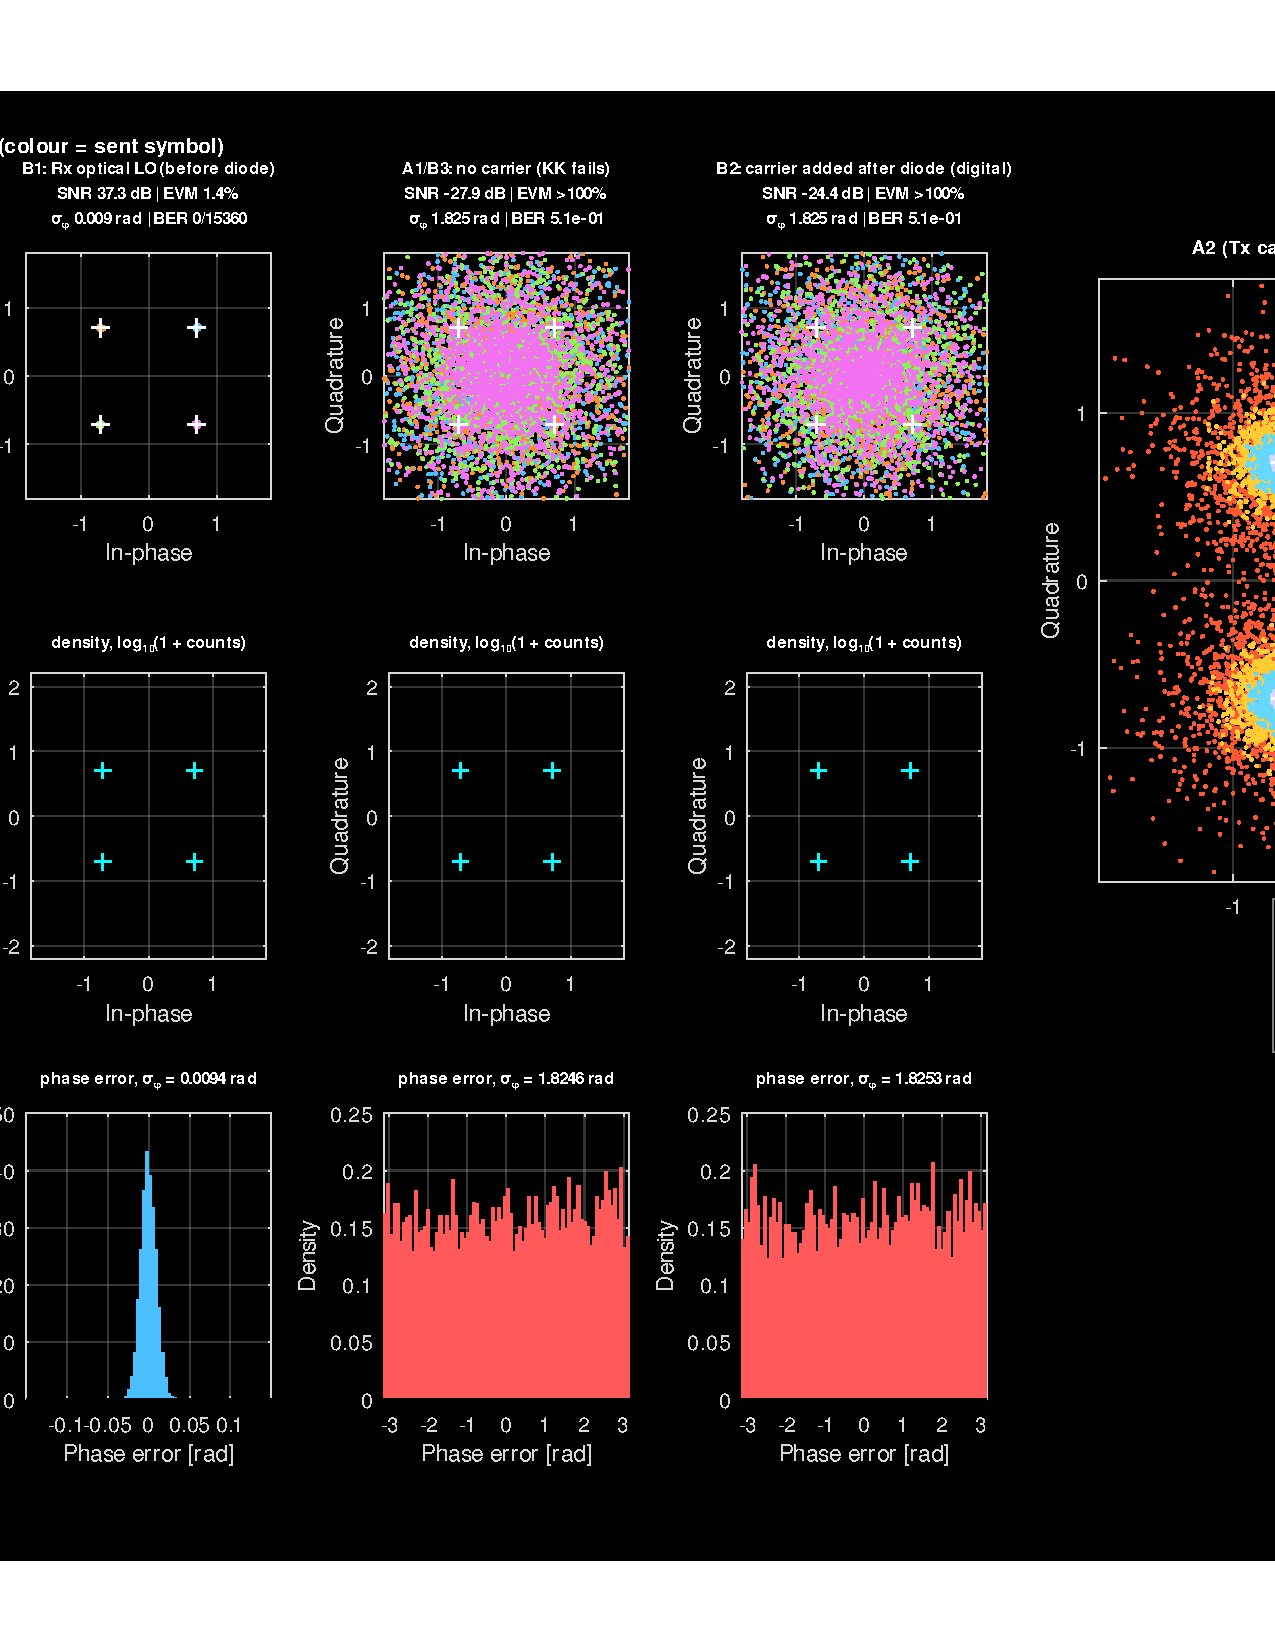
\includegraphics[width=\textwidth]{figs/fig36.pdf}
\caption{QPSK constellation study at $y=A_0$. Columns 1--4: A2, B1, A1/B3 and B2, each with the constellation (colour = transmitted symbol), a density map and the phase-error distribution. Right: A2 at $y/A_0=1$, 0.1, 0.03 and 0.01.}
\end{figure}

\begin{table}[h]
\centering
\caption{Constellation study at $y=A_0$, QPSK (7680 payload symbols, 15\,360 bits)}
\begin{tabular}{|l|c|c|c|c|}
\hline
\textbf{Configuration} & \textbf{SNR} & \textbf{EVM} & \textbf{BER} & $\boldsymbol{\sigma_\phi}$\\\hline
A2 TX carrier & 31.1\,dB & 2.8\,\% & 0/15\,360 & 0.020\,rad\\\hline
B1 RX LO (ideal) & 37.3\,dB & 1.4\,\% & 0/15\,360 & 0.009\,rad\\\hline
A1/B3 no carrier & $-27.9$\,dB & $>100$\,\% & 0.51 & 1.82\,rad\\\hline
B2 carrier added after detection & $-24.4$\,dB & $>100$\,\% & 0.51 & 1.83\,rad\\\hline
\end{tabular}
\end{table}

Configurations A2 and B1 both produce clean QPSK constellations, confirming that KK phase retrieval works whenever a carrier is present at the photodiode input, whether it arrived through the channel (A2) or was added locally (B1). A2 agrees with the analytic SNR (31.05\,dB). B1 is 6.2\,dB better because all of the transmit power carries data and its LO is ideal; this is the CSPR penalty of the transmitter carrier, measured against a receiver LO that has no frequency offset, no phase noise and no polarisation mismatch. With a realistic LO (100\,MHz residual offset after locking, 200\,kHz combined linewidth) and the same frequency and phase recovery as A2, B1 is still 4.2\,dB better on-axis and 6.9--8.7\,dB better at $y\le0.1A_0$, because its fixed LO power keeps the beat signal above thermal noise while the transmitted carrier fades with the data. The case for the transmitter carrier therefore rests on the hardware it avoids, not on SNR. Configurations A1/B3 and B2 fail completely: the BER is 0.5 and the phase error is spread over $[-\pi,\pi]$. Square-law detection $I=\eta|E|^2$ destroys the optical phase; the Hilbert-transform relation (eq.~3.7) recovers it only if a dominant carrier is present in the optical field \emph{before} detection. Adding the carrier level digitally afterwards (B2) cannot restore information that the photocurrent no longer contains.

\subsection{Detector Radius Sensitivity}

The detector radius $w_d$ appears in the peak collected fraction $A_0=2w_d^2/w_z^2$ and therefore directly controls the on-axis received power. Following the supervisor's guidance, $w_d$ is set 20--50\,\% below the transmitter beam waist $w_0=0.1$\,m, which motivates a sweep from 0.04\,m to 0.10\,m. The ergodic QPSK rate rises from 11.46\,Gbps at $w_d=0.04$\,m to 14.09\,Gbps at $w_d=0.10$\,m; the default $w_d=0.07$\,m gives 13.18\,Gbps, about 94\,\% of the rate at the largest radius in the sweep. The rate keeps increasing with $w_d$.

\begin{figure}[h]
\centering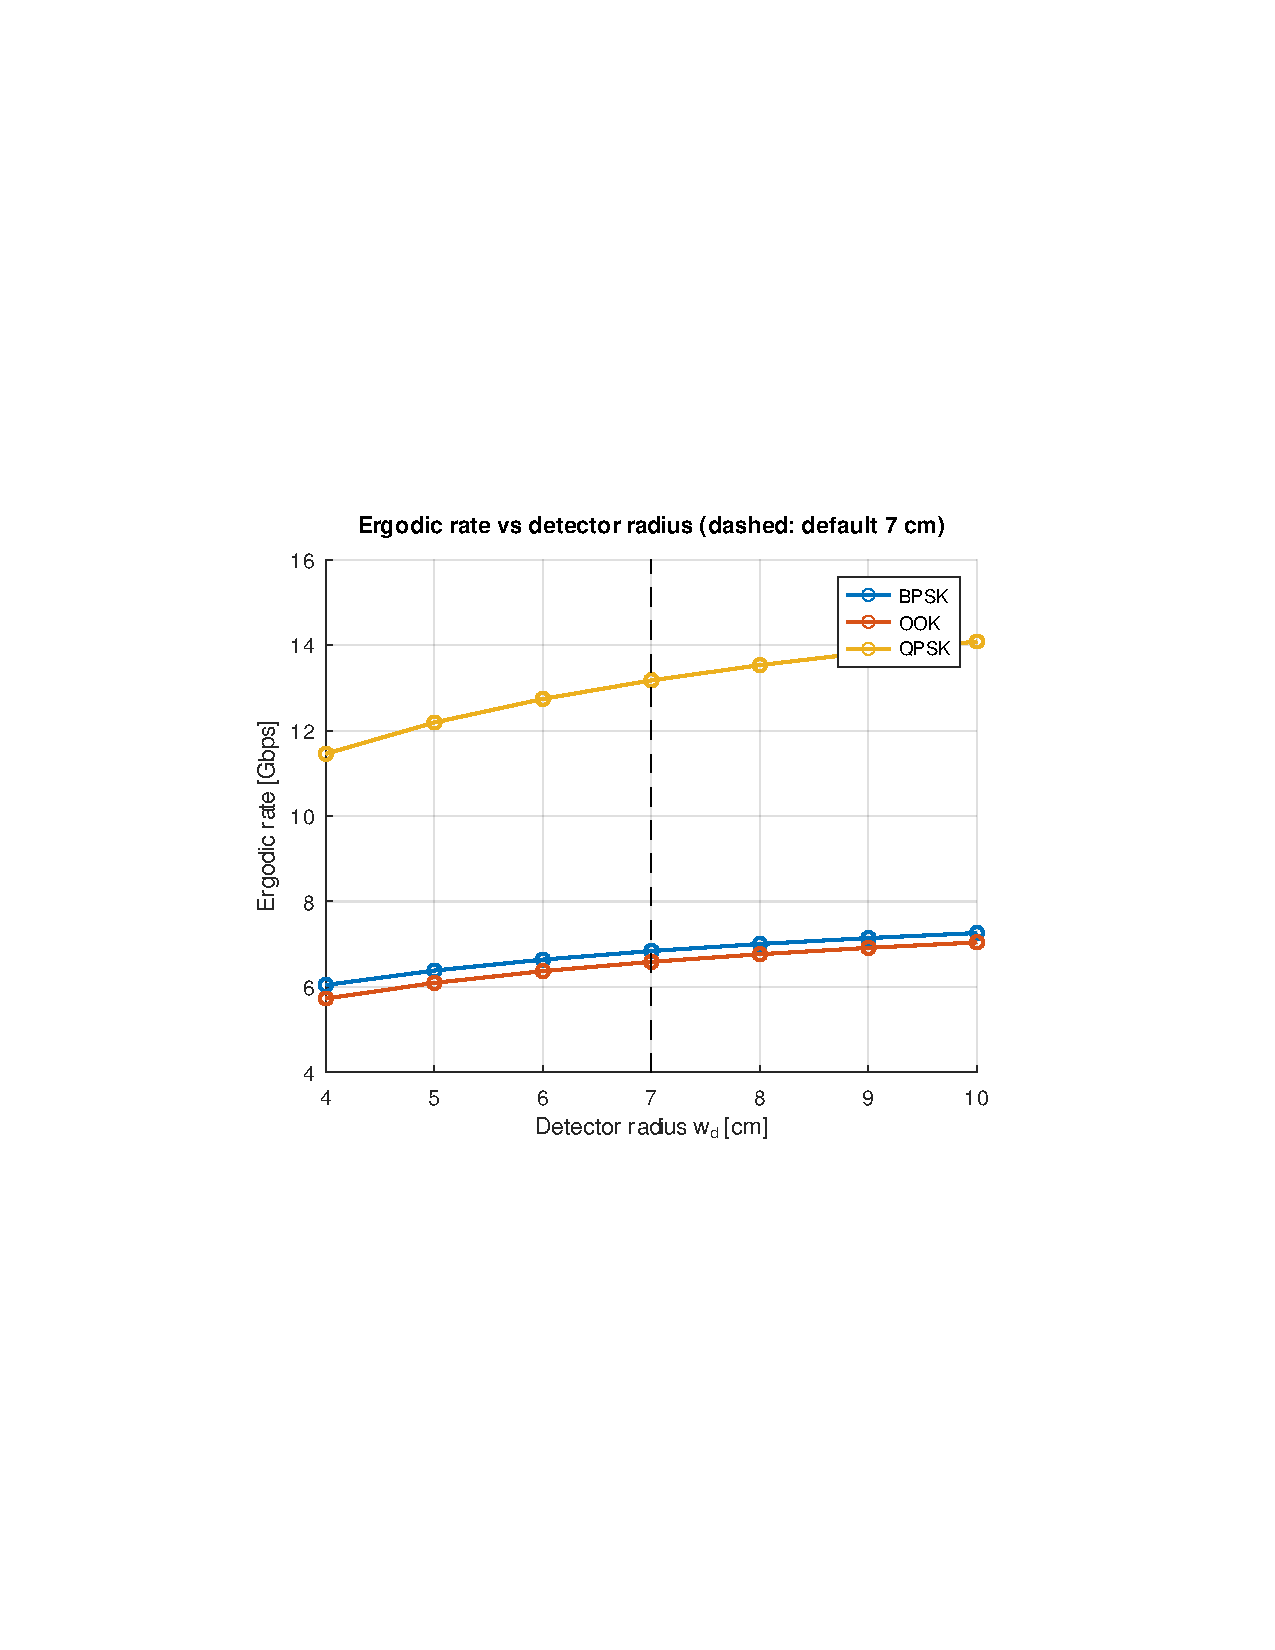
\includegraphics[width=0.85\textwidth]{figs/fig38.pdf}
\caption{Ergodic rate vs detector radius $w_d$ for all three modulation formats. Vertical dashed line: default $w_d=0.07$\,m. The rate increases monotonically with $w_d$ but with diminishing returns above $w_d\approx0.08$\,m.}
\end{figure}

\subsection{ITU-T C-Band Wavelength Comparison}

The ITU-T C-band spans 1530--1565\,nm (191.56--195.94\,THz). At the long-wavelength edge (1565\,nm) the beam divergence is slightly larger ($w_z=4.98$\,m vs 4.87\,m), which reduces $A_0$ from $4.13\times10^{-4}$ to $3.95\times10^{-4}$. However, the pointing shape parameter $\alpha$ increases from 0.201 to 0.210, which means the fading distribution is slightly less severe. These two effects approximately cancel: the ergodic QPSK rate changes from 13.18\,Gbps (1530\,nm) to 13.45\,Gbps (1565\,nm), a difference of about 2\,\% (2.3\,\% at $P_T=0.1$\,W).

\begin{figure}[h]
\centering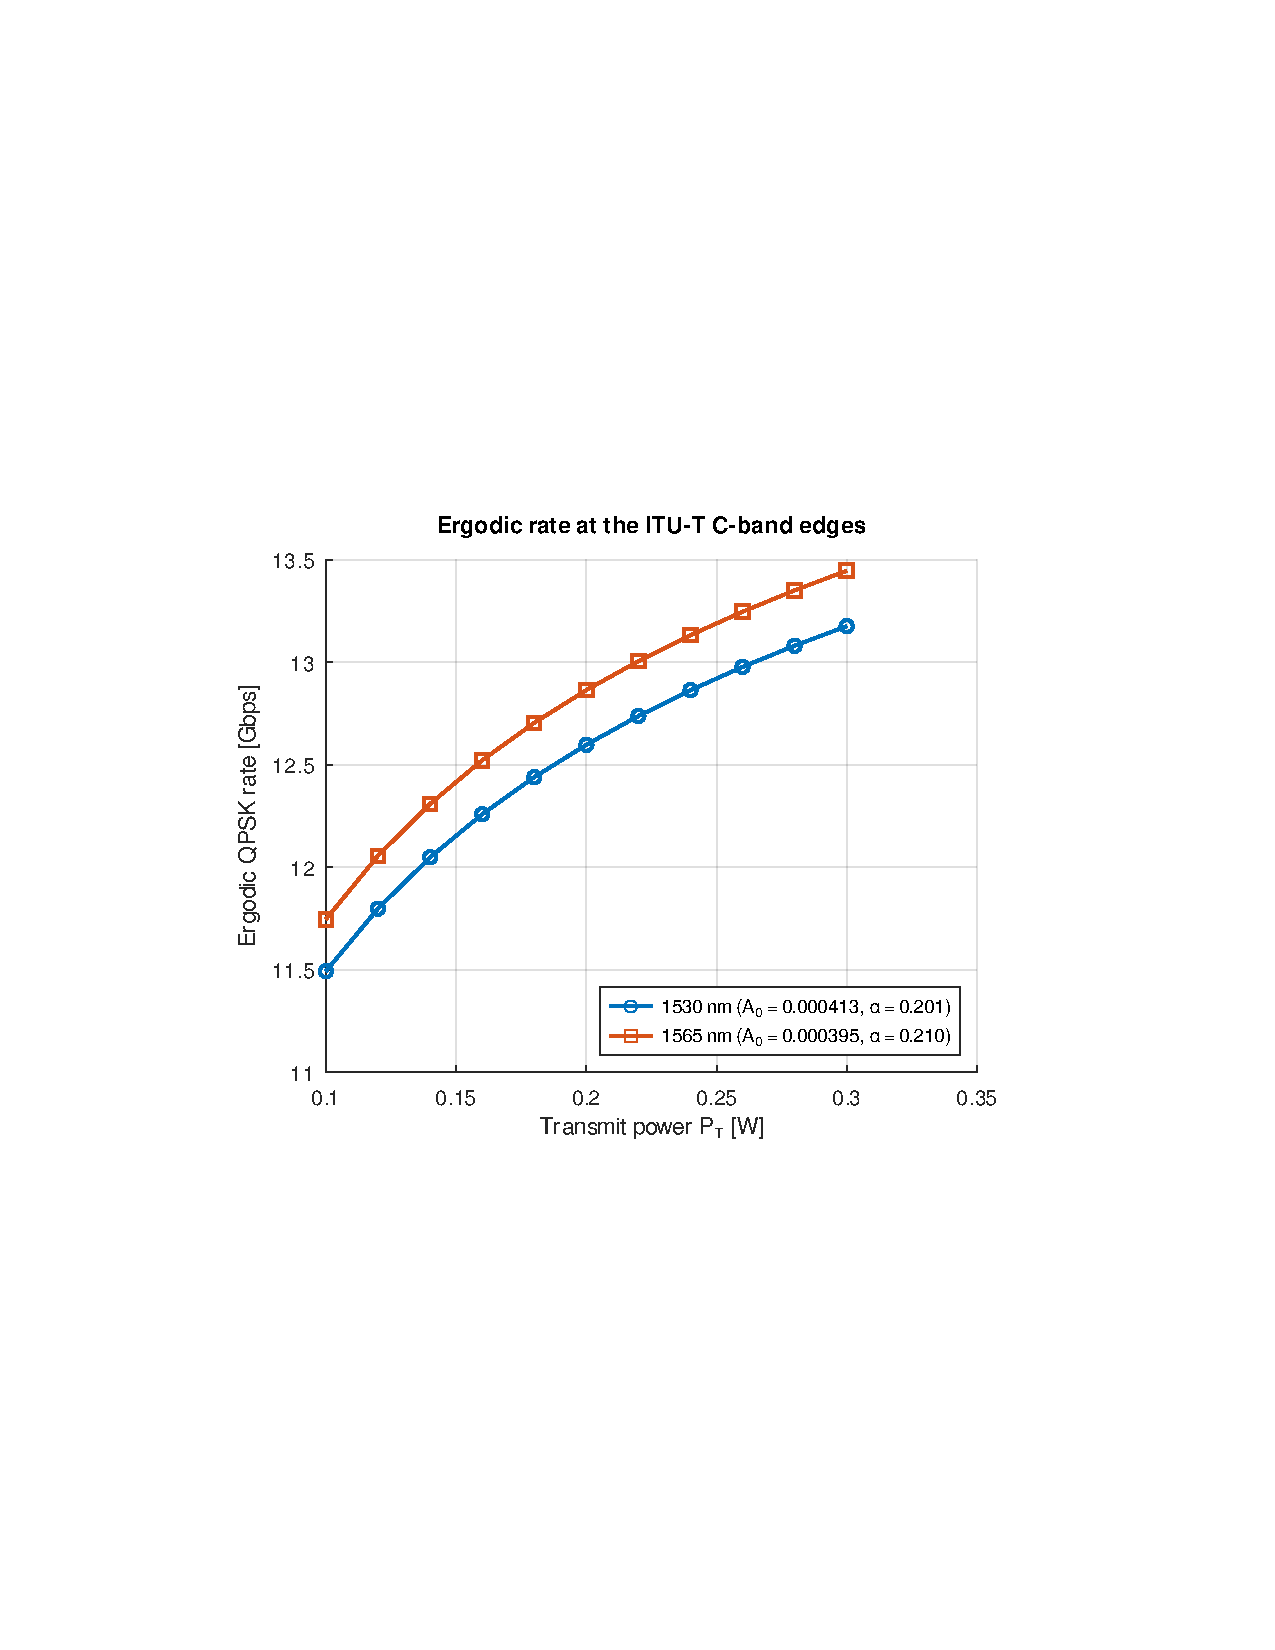
\includegraphics[width=0.85\textwidth]{figs/fig39.pdf}
\caption{Ergodic rate vs transmit power $P_T$ at the two ITU-T C-band edges: 1530\,nm and 1565\,nm. The 1565\,nm curve is slightly higher due to the more favourable $\alpha$ despite lower $A_0$. The difference is about 2\,\% across the power range.}
\end{figure}

\section{Rationale: Transmitter-Side Carrier vs Receiver-Side Local Oscillator}

Kramers--Kronig receivers were originally proposed for fibre-optic links, where the CW carrier can be placed either at the transmitter (co-propagating with the data) or at the receiver (as a local oscillator, LO). Both configurations recover the full optical field from a single photodiode, but they differ sharply in what the receiver must provide. This section compares the two options for the inter-satellite link scenario and motivates the choice of a transmitter-side carrier used throughout this chapter.

\subsection{Receiver-Side LO}

In the receiver-LO configuration the transmitter sends only the SSB data signal at full power $P_T$. The receiver mixes the incoming signal with a locally generated CW laser before the photodiode. The LO power can be chosen freely and made large, so the cross-beat current is proportional to $\sqrt{P_{LO}P_s}$ with an arbitrarily strong $P_{LO}$. This gives the architecture several advantages:

\begin{itemize}
\item \textbf{No CSPR penalty.} The full transmit power carries data; there is no power budget split between carrier and signal.
\item \textbf{Shot-noise-limited sensitivity.} A strong LO lifts the beat current well above thermal noise, approaching coherent-receiver performance from a single photodiode.
\item \textbf{No minimum-phase constraint.} The carrier power is set at the receiver and can always be made large enough; the PAPR of the transmitted signal is irrelevant to phase reconstruction.
\end{itemize}

However, in a free-space inter-satellite link these advantages come at significant cost:

\begin{itemize}
\item \textbf{Frequency locking.} The LO laser must be offset-locked to the transmitter laser to within a fraction of $B$. Two independent lasers on different spacecraft, each subject to mechanical vibration and thermal drift, require either an optical phase-locked loop (OPLL) or a digital frequency-offset estimator with $\ge$10-bit ADC and real-time DSP.

\item \textbf{Doppler compensation.} For a 550\,km LEO constellation the carrier Doppler shift can reach $\pm9.9$\,GHz. The LO must track this shift in real time, which demands a widely tunable laser or an acousto-optic frequency shifter, adding mass, power and complexity.

\item \textbf{Phase noise.} The transmitter and receiver lasers have independent phase-noise processes. The beat signal carries their sum, which must be tracked by carrier-phase recovery DSP. For linewidths above $\sim100$\,kHz the cycle-slip rate becomes significant at the symbol rates considered here.

\item \textbf{Polarisation.} The received field arrives in an arbitrary and time-varying polarisation state (due to spacecraft rotation and optical-bench flexure). A single photodiode with LO mixing sees only the projection onto the LO's polarisation; recovering the full signal requires a polarisation-diversity receiver (two photodiodes, a polarisation beam splitter and Stokes-parameter tracking), roughly doubling the front-end hardware.
\end{itemize}

\subsection{Transmitter-Side Carrier}

In the transmitter-carrier configuration the CW tone is generated from the \emph{same laser} as the data signal and is transmitted in the same spatial mode, same polarisation and same beam. At the receiver, a single photodiode performs square-law detection; the KK algorithm recovers the optical field entirely in digital signal processing.

Because the carrier and data share the same laser and propagation path:

\begin{itemize}
\item \textbf{Phase noise cancels.} The laser phase $\theta_L(t)$ is common to the carrier and the signal. In the photocurrent $I(t)=\eta|E_{Rx}|^2$, the phase drops out. No carrier-phase recovery is needed.

\item \textbf{Doppler cancels.} The Doppler shift $\phi_D(t)$ affects the carrier and the signal identically. The cross-beat current sees only the difference, which is the fixed SSB offset $f_{sh}$. No Doppler tracking or tunable laser is required.

\item \textbf{Polarisation cancels.} Whatever polarisation rotation the channel imposes acts on the carrier and signal equally. The photocurrent is insensitive to the absolute polarisation state. A single photodiode suffices.

\item \textbf{No LO laser.} The receiver is simply a photodiode (optionally preceded by an EDFA) followed by an ADC and DSP. There is no second laser, no frequency-locking loop, no polarisation optics.
\end{itemize}

The price is the CSPR power penalty. At $\kappa=12$\,dB, only $P_s/P_T=1/(1+\kappa)\approx6\,\%$ of the transmit power carries information; the rest is spent on the carrier. Additionally, the minimum-phase condition $\kappa>\mathrm{PAPR}_s$ imposes a floor on the CSPR, limiting the amount of power that can be shifted from carrier to data.

\subsection{Trade-off Summary}

\begin{table}[h]
\centering
\caption{Comparison of transmitter-side carrier and receiver-side LO for OISL}
\begin{tabular}{|p{4.0cm}|p{5.0cm}|p{5.0cm}|}
\hline
\textbf{Attribute} & \textbf{TX-side carrier} & \textbf{RX-side LO}\\\hline
Frequency locking & Not needed & Required (OPLL or DSP)\\\hline
Doppler tracking & Not needed & $\pm9.9$\,GHz tuning for LEO\\\hline
Phase-noise tolerance & Immune (common path) & Limited by combined linewidth\\\hline
Polarisation control & Not needed & Diversity receiver or tracking\\\hline
Receiver hardware & Photodiode + EDFA + ADC & Photodiode + tunable laser + PBS + 2 ADCs\\\hline
Transmit power efficiency & $1/(1+\kappa)\approx6\,\%$ at 12\,dB & 100\,\% (no carrier overhead)\\\hline
Sensitivity (pre-amp) & ASE limited ($-28.6$\,dBm QPSK) & Near shot-noise limited\\\hline
Min-phase constraint & $\kappa>\mathrm{PAPR}_s$ required & None\\\hline
DSP complexity & KK: $\ln$, Hilbert, matched filter & Freq.\ offset + phase recovery + pol.\ demux\\\hline
\end{tabular}
\end{table}

For a mass- and power-constrained satellite terminal, the transmitter-side carrier trades about 6\,dB of SNR (6.2\,dB against an ideal receiver LO in Section~3.2.1) for the complete elimination of the LO laser, frequency-locking loop, polarisation optics and Doppler-tracking hardware. The resulting receiver is a single photodiode with digital back-end, which is the simplest coherent-capable architecture possible. The CSPR power penalty is partially recovered by the pre-amplifier (which boosts carrier and signal equally) and could be reduced further by operating near the optimal CSPR found by waveform simulation (7--9\,dB, a gain of 2--3\,dB over 12\,dB). In constellations where the link budget has margin (e.g.\ short LEO--LEO links with $<2000$\,km range), the power penalty is acceptable and the hardware simplification is decisive.
